\documentclass[pdflatex,compress,mathserif]{beamer}

%\usetheme[dark,framenumber,totalframenumber]{ElektroITK}
\usetheme[darktitle,framenumber,totalframenumber]{ElektroITK}

\usepackage[utf8]{inputenc}
\usepackage[T1]{fontenc}
\usepackage{lmodern}
\usepackage[bahasai]{babel}
\usepackage{amsmath}
\usepackage{amsfonts}
\usepackage{amssymb}
\usepackage{graphicx}
\usepackage{multicol}

\newcommand*{\Scale}[2][4]{\scalebox{#1}{$#2$}}%

\title{Pengolahan Sinyal Digital}
\subtitle{Inverse Transformasi Z}

\author{Tim Dosen Pengampu}

\begin{document}

\maketitle

\begin{frame}
	\frametitle{Transformasi Z}
	\begin{itemize}
		\item Persamaan Transformasi Z:
		\begin{equation}
			X(z) = \sum\limits_{n=-\infty}^{+\infty} x(z)z^{-n}
		\end{equation}
	\end{itemize}
\end{frame}

\begin{frame}
	\frametitle{Inverse Transformasi Z}
	Metode-metode:
	\begin{enumerate}
		\item Metode Inspeksi
		\begin{equation}
			a^nu(n) \leftrightarrow \frac{1}{1-az^{-1}};\quad|z|>|a|
		\end{equation}
		\begin{equation}
			-a^nu(n) \leftrightarrow \frac{1}{1-az^{-1}};\quad|z|<|a|
		\end{equation}
		dst.
	\end{enumerate}
\end{frame}

\begin{frame}{Inverse Transformasi Z}
	\begin{enumerate}
		\setcounter{enumi}{1}
		\item Power Series
		\begin{equation*}
			X(z)= \frac{1}{1-az^{-1}};\quad|z|>|a|
		\end{equation*}
		\begin{center}
			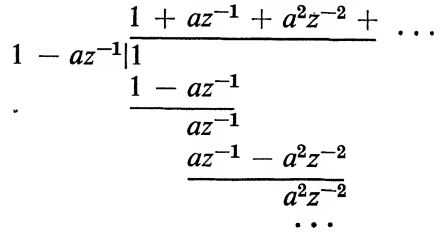
\includegraphics[width=0.6\linewidth]{img/img01}
		\end{center}
	\end{enumerate}
\end{frame}

\begin{frame}{Inverse Transformasi Z}
	\begin{enumerate}
		\setcounter{enumi}{1}
		\item Power Series
		\begin{equation*}
		X(z)= \frac{1}{1-az^{-1}};\quad|z|<|a|
		\end{equation*}
		\begin{center}
			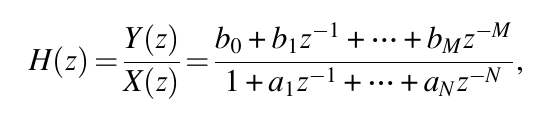
\includegraphics[width=0.6\linewidth]{img/img02}
		\end{center}
	\end{enumerate}
\end{frame}

\end{document}